%
% strukturen.tex
%
% (c) 2021 Prof Dr Andreas Müller, OST Ostschweizer Fachhochschule
%
\section{Algebraische Strukturen
\label{buch:section:algebraische-Strukturen}}
Im Laufe der Definition der Vektorräume $\Bbbk^n$ und der
Operationen für die Matrizen in $M_{m\times n}(\Bbbk)$ haben
wir eine ganze Reihe von algebraischen Strukturen kennengelernt.
Nicht immer sind alle Operationen verfügbar, in einem Vektorraum
gibt es normalerweise kein Produkt.
Und bei der Konstruktion des Zahlensystems wurde gezeigt, dass
additive oder multiplikative Inverse nicht selbstverständlich
sind.
Sinnvolle Mathematik lässt sich aber erst betreiben, wenn zusammen
mit den vorhandenen Operationen auch einige Regeln erfüllt sind.
Die schränkt die Menge der sinnvollen Gruppierungen von Eigenschaften
ein.
In diesem Abschnitten sollen diesen sinnvollen Gruppierungen von
Eigenschaften Namen gegeben werden.

%
% gruppen.tex
%
% (c) 2021 Prof Dr Andreas Müller, Hochschule Rapeprswil
%
\subsection{Gruppen
\label{buch:grundlagen:subsection:gruppen}}
Die kleinste sinnvolle Struktur ist die einer Gruppe.
Eine solche besteht aus einer Menge $G$ mit einer Verknüpfung,
die additiv
\begin{align*}
G\times G \to G&: (g,h) = gh
\intertext{oder multiplikativ }
G\times G \to G&: (g,h) = g+h
\end{align*}
geschrieben werden kann.
Ein Element $0\in G$ heisst {\em neutrales Element} bezüglich der additiv
geschriebenen Verknüpfung falls $0+x=x$ für alle $x\in G$.
\index{neutrales Element}%
Ein Element $e\in G$ heisst neutrales Element bezüglich der multiplikativ 
geschriebneen Verknüpfung, wenn $ex=x$ für alle $x\in G$.
In den folgenden Definitionen werden wir immer die multiplikative
Schreibweise verwenden, für Fälle additiv geschriebener siehe auch die
Beispiele weiter unten.

\begin{definition}
\index{Gruppe}%
Ein {\em Gruppe}
\index{Gruppe}%
ist eine Menge $G$ mit einer Verknüfung mit folgenden
Eigenschaften:
\begin{enumerate}
\item
Die Verknüpfung ist assoziativ: $(ab)c=a(bc)$ für alle $a,b,c\in G$.
\item
Es gibt ein neutrales Element $e\in G$
\item
Für jedes Element $g\in G$ gibt es ein Element $h\in G$ mit 
$hg=e$.
\end{enumerate}
Das Element $h$ heisst auch das Inverse Element zu $g$.
\end{definition}

Falls nicht jedes Element invertierbar ist, aber wenigstens ein neutrales
Element vorhanden ist, spricht man von einem {\em Monoid}.
\index{Monoid}%
Hat man nur eine Verknüpfung, spricht man oft von einer {\em Halbruppe}.
\index{Halbgruppe}%

\begin{definition}
Eine Gruppe $G$ heisst abelsch, wenn $ab=ba$ für alle $a,b\in G$.
\end{definition}

Additiv geschrieben Gruppen werden immer als abelsch angenommen,
multiplikativ geschrieben Gruppen können abelsch oder nichtabelsch sein.

\subsubsection{Beispiele von Gruppen}

\begin{beispiel}
Die Menge $\mathbb{Z}$ mit der Addition ist eine additive Gruppe mit
dem neutralen Element $0$.
Das additive Inverse eines Elementes $a$ ist $-a$.
\end{beispiel}

\begin{beispiel}
Die von Null verschiedenen Elemente $\Bbbk^*$ eines Zahlekörpers bilden
bezüglich der Multiplikation eine Gruppe mit neutralem Element $1$.
Das multiplikative Inverse eines Elementes $a\in \Bbbk$ mit $a\ne 0$
ist $a^{-1}=\frac1{a}$.
\end{beispiel}

\begin{beispiel}
Die Vektoren $\Bbbk^n$ bilden bezüglich der Addition eine Gruppe mit
dem Nullvektor als neutralem Element.
Betrachtet man $\Bbbk^n$ als Gruppe, verliert man die Multiplikation
mit Skalaren aus den Augen.
$\Bbbk^n$ als Gruppe zu bezeichnen ist also nicht falsch, man
verliert dadurch aber 
\end{beispiel}

\begin{beispiel}
Die Menge aller quadratischen $n\times n$-Matrizen $M_n(\Bbbk)$ ist
eine Gruppe bezüglich der Addition mit der Nullmatrix als neutralem
Element.
Bezügich der Matrizenmultiplikation ist $M_n(\Bbbk)$ aber keine
Gruppe, da sich die singulären Matrizen nicht inverieren lassen.
Die Menge der invertierbaren Matrizen
\[
\operatorname{GL}_n(\Bbbk)
=
\{
A\in M_n(\Bbbk)\;|\; \text{$A$ invertierbar}
\}
\]
ist bezüglich der Multiplikation eine Gruppe.
Die Gruppe $\operatorname{GL}_n(\Bbbk)$ ist eine echte Teilmenge 
von $M_n(\Bbbk)$, die Addition und Multiplikation führen im Allgemeinen
aus der Gruppe heraus, es gibt also keine Mögichkeit, in der Gruppe
$\operatorname{GL}_n(\Bbbk)$ diese Operationen zu verwenden.
\end{beispiel}

\subsubsection{Einige einfache Rechenregeln in Gruppen}
Die Struktur einer Gruppe hat bereits eine Reihe von
Einschränkungen zur Folge.
Zum Beispiel sprach die Definition des neutralen Elements $e$ nur von
Produkten der Form $ex=x$, nicht von Produkten $xe$.
Und die Definition des inversen Elements $h$ von $g$ hat nur
verlangt, dass $gh=e$, es wurde nichts gesagt über das Produkt $hg$.

\begin{satz}
\label{buch:vektorenmatrizen:satz:gruppenregeln}
Ist $G$ eine Gruppe mit neutralem Element $e$, dann gilt
\begin{enumerate}
\item
$xe=x$ für alle $x\in G$
\item
Es gibt nur ein neutrales Element.
Wenn also $f\in G$ mit $fx=x$ für alle $x\in G$, ist dann folgt $f=e$.
\item 
Wenn $hg=e$ gilt, dann auch $gh=e$ und $h$ ist durch $g$ eindeutig bestimmt.
\end{enumerate}
\end{satz}

\begin{proof}[Beweis]
Wir beweisen als Erstes den ersten Teil der Eigenschaft~3.
Sei $h$ die Inverse von $g$, also $hg=e$.
Sei weiter $i$ die Inverse von $h$, also $ih=e$.
Damit folgt jetzt
\[
g
=
eg
=
(ih)g
=
i(hg)
=
ie.
\]
Wende man dies auf das Produkt $gh$ an, folgt
\[
gh
=
(ie)h
=
i(eh)
=
ih
=
e
\]
Es ist also nicht nur $hg=e$ sondern immer auch $gh=e$.

Für eine Inverse $h$ von $g$ folgt
\[
ge
=
g(hg)
=
(gh)g
=
eg
=
g,
\]
dies ist die Eigenschaft~1.

Sind $f$ und $e$ neutrale Elemente, dann folgt
\[
f = fe = e
\]
aus der Eigenschaft~1.

Schliesslich sei $x$ ein beliebiges Inverses von $g$, dann ist
$xg=e$, dann folgt
$x=xe=x(gh)=(xg)h = eh = h$, es gibt also nur ein Inverses von $g$.
\end{proof}

Diesem Problem sind wir zum Beispiel auch in
Abschnitt~\ref{buch:grundlagen:subsection:gleichungssyteme}
begegnet, wo wir nur gezeigt haben, dass $AA^{-1}=E$ ist.
Da aber die invertierbaren Matrizen eine Gruppe
bilden, folgt jetzt aus dem Satz automatisch, dass auch $A^{-1}A=E$.

\subsubsection{Homomorphismen} \label{buch:gruppen:subsection:homomorphismen}
Lineare Abbildung zwischen Vektorräumen zeichnen sich dadurch aus,
dass sie die algebraische Struktur des Vektorraumes respektieren.
Für eine Abbildung zwischen Gruppen heisst dies, dass die Verknüpfung,
das neutrale Element und die Inverse respektiert werden müssen.

\begin{definition}
Ein Abbildung $\varphi\colon G\to H$ zwischen Gruppen heisst ein
{\em Homomorphismus}, wenn 
$\varphi(g_1g_2)=\varphi(g_1)\varphi(g_2)$ für alle $g_1,g_2\in G$ gilt.
\index{Homomorphismus}%
\end{definition}

Der Begriff des Kerns einer linearen Abbildung lässt sich ebenfalls auf
die Gruppensituation erweitern.
Auch hier ist der Kern der Teil der Gruppe, er unter dem 
Homomorphismus ``unsichtbar'' wird.

\begin{definition}
Ist $\varphi\colon G\to H$ ein Homomorphisus, dann ist
\[
\ker\varphi
=
\{g\in G\;|\; \varphi(g)=e\}
\]
eine Untergruppe.
\index{Kern}%
\end{definition}

\subsubsection{Normalteiler}
Der Kern eines Homomorphismus ist nicht nur eine Untergruppe, er erfüllt
noch eine zusätzliche Bedingung. 
Für jedes $g\in G$ und $h\in\ker\varphi$ gilt 
\[
\varphi(ghg^{-1})
=
\varphi(g)\varphi(h)\varphi(g^{-1})
=
\varphi(g)\varphi(g^{-1})
=
\varphi(gg^{-1})
=
\varphi(e)
=
e
\qquad\Rightarrow\qquad
ghg^{-1}\in\ker\varphi.
\]
Der Kern wird also von der Abbildung $h\mapsto ghg^{-1}$,
der {\em Konjugation} in sich abgebildet.

\begin{definition}
Eine Untergruppe $H \subset G$ heisst ein {\em Normalteiler},
geschrieben $H \triangleleft G$
wenn $gHg^{-1}\subset H$ für jedes $g\in G$.
\index{Normalteiler}
\end{definition}

Die Konjugation selbst ist ebenfalls keine Unbekannte, sie ist uns
bei der Basistransformationsformel schon begegnet.
Die Tatsache, dass $\ker\varphi$ unter Konjugation erhalten bleibt,
kann man also interpretieren als eine Eigenschaft, die unter
Basistransformation erhalten bleibt.

\subsubsection{Faktorgruppen}
Ein Unterraum $U\subset V$ eines Vektorraumes gibt Anlass zum
Quotientenraum, der dadurch entsteht, dass man die Vektoren in $U$
zu $0$ kollabieren lässt.
Eine ähnliche Konstruktion könnte man für eine Untergruppe $H \subset G$
versuchen.
Man bildet also wieder die Mengen von Gruppenelementen, die sich um
ein Elemente in $H$ unterscheiden.
Man kann diese Mengen in der Form $gH$ mit $g\in G$ schreiben.

Man möchte jetzt aber auch die Verknüpfung für solche Mengen 
definieren, natürlich so, dass $g_1H\cdot g_2H = (g_1g_2)H$ ist.
Da die Verknüpfung nicht abelsch sein muss, entsteht hier
ein Problem.
Für $g_1=e$ folgt, dass $Hg_2H=g_2H$ sein muss.
Das geht nur, wenn $Hg_2=g_2H$ oder $g_2Hg_2^{-1}=H$ ist, wenn
also $H$ ein Normalteiler ist.

\begin{definition}
Für eine Gruppe $G$ mit Normalteiler  $H\triangleleft G$ ist die
Menge
\[
G/H = \{ gH \;|\; g\in G\}
\]
eine Gruppe mit der Verknüpfung $g_1H\cdot g_2H=(g_1g_2)H$.
$G/H$ heisst {\em Faktorgruppe} oder {\em Quotientengruppe}.
\index{Faktorgruppe}%
\index{Quotientengruppe}%
\end{definition}

Für abelsche Gruppen ist die Normalteilerbedingung keine zusätzliche
Einschränkung, jeder Untergruppe ist auch ein Normalteiler.

\begin{beispiel}
Die ganzen Zahlen $\mathbb{Z}$ bilden eine abelsche Gruppe und
die Menge der Vielfachen von $n$
$n\mathbb{Z}\subset\mathbb{Z}$ ist eine Untergruppe.
Da $\mathbb{Z}$ abelsch ist, ist $n\mathbb{Z}$ ein Normalteiler
und die Faktorgruppe $\mathbb{Z}/n\mathbb{Z}$ ist wohldefiniert.
Nur die Elemente
\[
0+n\mathbb{Z},
1+n\mathbb{Z},
2+n\mathbb{Z},
\dots
(n-1)+n\mathbb{Z}
\]
sind in der Faktorgruppe verschieden.
Die Gruppe $\mathbb{Z}/n\mathbb{Z}$ besteht also aus den Resten
bei Teilung durch $n$.
Diese Gruppe wird in Kapitel~\ref{buch:chapter:endliche-koerper}
genauer untersucht.
\end{beispiel}

Das Beispiel suggeriert, dass man sich die Elemente von $G/H$
als Reste vorstellen kann.

\subsubsection{Darstellungen}
Abstrakt definierte Gruppen können schwierig zu verstehen sein.
Oft hilft es, wenn man eine geometrische Darstellung der Gruppenoperation
finden kann.
Die Gruppenelemente werden dann zu umkehrbaren linearen Operationen
auf einem geeigneten Vektorraum.

\begin{definition}
\label{buch:vektorenmatrizen:def:darstellung}
Eine Darstellung einer Gruppe $G$ ist ein Homomorphismus 
$G\to\operatorname{GL}_(\mathbb{R})$.
\index{Darstellung}
\end{definition}

\begin{beispiel}
Die Gruppen $\operatorname{GL}_n(\mathbb{Z})$,
$\operatorname{SL}_n(\mathbb{Z})$ oder $\operatorname{SO}(n)$ 
sind alle Teilmengen von $\operatorname{GL}_n(\mathbb{R}$.
Die Einbettungsabbildung $G\hookrightarrow \operatorname{GL}_n(\mathbb{R})$
ist damit automatisch eine Darstellung, sie heisst auch die
{\em reguläre Darstellung} der Gruppe $G$.
\index{reguläre Darstellung}
\end{beispiel}

In Kapitel~\ref{buch:chapter:permutationen} wird gezeigt, 
dass Permutationen einer endlichen eine Gruppe bilden und wie
sie durch Matrizen dargestellt werden können.







%
% ringe.tex -- Grundlegende Konstruktionen für Ringe
%
% (c) 2021 Prof Dr Andreas Müller, OST Ostschweizer Fachhochschule
%
\subsection{Ringe und Moduln
\label{buch:grundlagen:subsection:ringe}}
\rhead{Ringe}
Die ganzen Zahlen haben ausser der Addition mit neutralem Element $0$
auch noch eine Multiplikation mit dem neutralen Element $1$.
Die Multiplikation ist aber nicht immer invertierbar und zwar
nicht nur für $0$.
Eine ähnliche Situation haben wir bei $M_n(\Bbbk)$ angetroffen.
$M_n(\Bbbk)$ ist eine zunächst eine Gruppe bezüglich der Addition,
hat aber auch noch eine Multiplikation, die nicht immer umkehrbar ist.
Diese Art von Struktur nennt man einen Ring.

\subsubsection{Definition eines Rings}

\begin{definition}
\index{Ring}%
Eine Menge $R$ mit einer additiven Operation $+$ mit neutralem Element
$0$ und einer multiplikativ geschriebenen Operation $\cdot$ heisst ein
{\em Ring}, wenn folgendes gilt.
\begin{enumerate}
\item
$R$ ist eine Gruppe bezüglich der Addition.
\item
$R\setminus\{0\}$ ist eine Halbgruppe.
\item
Es gelten die {\em Distributivgesetze}
\[
a(b+c)=ab+ac
\qquad\text{und}\qquad
(a+b)c=ac+bc
\]
für beliebige Elemente $a,b,c\in R$.
\index{Distributivgesetz}%
\end{enumerate}
\end{definition}

Die Distributivgesetze stellen sicher, dass man in $R$ beliebig
ausmultiplizieren kann.
Man kann also so rechnen kann, wie man sich das gewohnt ist.
Es stellt auch sicher, dass die Multiplikation mit $0$ immer $0$
ergibt, denn es ist
\[
r0 = r(a-a) = ra-ra=0.
\]

Man beachte, dass weder verlangt wurde, dass die Multiplikation
ein neutrales Element hat oder kommutativ ist.
Der Ring $\mathbb{Z}$ erfüllt beide Bedingungen.
Die Beispiele weiter unten werden zeigen, dass es auch Ringe gibt,
in denen die Multiplikation nicht kommutativ ist, die Multiplikation
kein neutrales Element hat oder beides.

\begin{definition}
\index{Ring mit Eins}%
Ein Ring $R$ heisst ein Ring mit Eins, wenn die Multiplikation ein
neutrales Element hat.
\end{definition}

\begin{definition}
\index{Ring!kommutativ}%
\index{kommutativer Ring}%
Ein Ring $R$ heisst kommutativ, wenn die Multiplikation kommutativ
ist.
\end{definition}

\subsubsection{Beispiele von Ringen}

\begin{beispiel}
Alle Zahlenkörper aus Kapitel~\ref{buch:chapter:zahlen} sind kommutative
Ringe mit Eins.
\end{beispiel}

\begin{beispiel}
Die Menge $c(\mathbb{Z})$ der Folgen $(a_n)_{n\in\mathbb{N}}$ mit
Folgengliedern in $\mathbb{Z}$ wird eine Ring, wenn man die Addition
und Multiplikation elementweise definiert, also
\begin{align*}
&\text{Addition:}
&
a+b&\text{\;ist die Folge mit Folgengliedern}&
(a+b)_n &= a_nb_n \quad\text{für alle $n\in\mathbb{N}$}
\\
&\text{Multiplikation:}
&
a\cdot b&\text{\;ist die Folge mit Folgengliedern}&
(a\cdot b)_n &=  a_nb_n \quad\text{für alle $n\in\mathbb{N}$}
\end{align*}
für $a,b\in c(\mathbb{Z})$.
Die Algebra ist kommutativ und hat die konstante Folge 
$u_n = 1\;\forall n$ als Eins.

Wir betrachten jetzt ein Unterring $c_0(\mathbb{Z})\subset c(\mathbb{Z})$
bestehend aus den Folgen, die nur für endlich viele Folgenglieder von
$0$ verschieden sind.
Für eine Folge $a\in c_0(\mathbb{Z})$ gibt es eine Zahl $N$ derart, dass
$a_n=0$ für $n\ge N$.
Die konstante Folge $u_n=1$, die in $c(\mathbb{Z})$ erfüllt diese
Bedingung nicht, die Eins des Ringes $c(\mathbb{Z})$ ist also nicht in
$c_0(\mathbb{Z})$.
$c_0(\mathbb{Z})$ ist immer noch ein Ring, aber er hat kein Eins.
\end{beispiel}

\begin{beispiel}
\begin{figure}
\centering
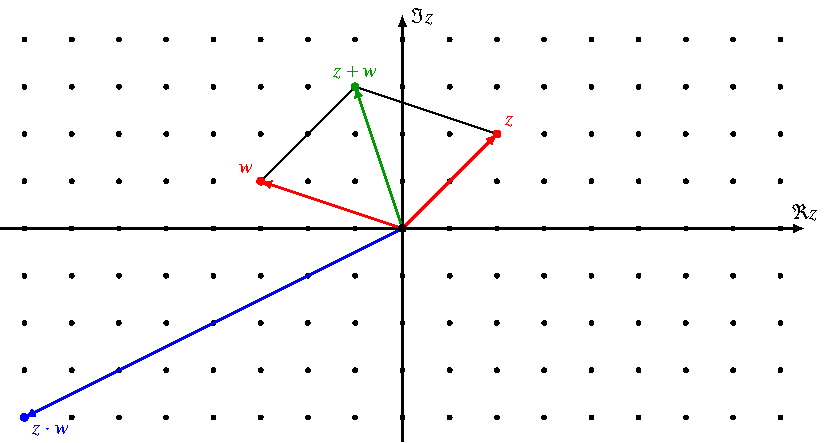
\includegraphics{chapters/10-vektorenmatrizen/images/gausszahlen.pdf}
%\begin{tikzpicture}[>=latex,thick,scale=0.8]
%\draw[->] (-8.5,0) -- (8.5,0) coordinate[label={$\Re z$}];
%\draw[->] (0,-4.5) -- (0,4.5) coordinate[label={right:$\Im z$}];
%\foreach \x in {-8,...,8}{
%	\foreach \y in {-4,...,4}{
%		\fill (\x,\y) circle[radius=0.05];
%	}
%}
%
%
%\coordinate (O) at (0,0);
%\coordinate (A) at (2,2);
%\coordinate (B) at (-3,1);
%\coordinate (C) at (-8,-4);
%\coordinate (D) at (-1,3);
%\draw[line width=0.5pt] (A)--(D)--(B);
%\draw[->,color=red] (O) -- (A);
%\draw[->,color=red] (O) -- (B);
%\draw[->,color=blue] (O) -- (C);
%\draw[->,color=darkgreen] (O) -- (D);
%\fill[color=red] (A) circle[radius=0.08];
%\fill[color=red] (B) circle[radius=0.08];
%\fill[color=blue] (C) circle[radius=0.08];
%\fill[color=darkgreen] (D) circle[radius=0.08];
%\fill[color=black] (O) circle[radius=0.08];
%\node[color=red] at (A) [above right] {$z$};
%\node[color=red] at (B) [above left] {$w$};
%\node[color=darkgreen] at (D) [above] {$z+w$};
%\node[color=blue] at (C) [below right] {$z\cdot w$};
%
%\end{tikzpicture}
\caption{Der Ring der ganzen Gausschen Zahlen besteht aus den ganzahligen
Gitterpunkten in der Gausschen Zahlenebene
\label{buch:vektorenmatrizen:fig:ganzgauss}}
\end{figure}
Die Menge
\[
\mathbb{Z} + i\mathbb{Z}
=
\{a+bi\;|\; a,b\in\mathbb{Z}\}
=
\mathbb{Z}[i]
\subset
\mathbb{C}
\]
ist eine Teilmenge von $\mathbb{C}$ und erbt natürlich die 
arithmetischen Operationen.
Die Summe zweier solcher Zahlen $a+bi\in\mathbb{Z}[i]$ und
$c+di\in\mathbb{Z}[i]$ ist
$(a+bi)+(c+di)=(a+c) + (b+d)i\in \mathbb{Z}[i]$, weil $a+c\in\mathbb{Z}$
und $b+d\in\mathbb{Z}$ ganze Zahlen sind.
Ebenso ist das Produkt dieser Zahlen
\(
(a+bi)(c+di)
=
(ac-bd) + (ad+bc)i
\in \mathbb{Z}[i]
\)
weil Realteil $ac-bd\in\mathbb{Z}$ und der Imaginärteil $ad+bc\in\mathbb{Z}$
ganze Zahlen sind.
Die Menge $\mathbb{Z}[i]$ ist also ein kommutative Ring mit Eins, er
heisst der Ring der ganzen {\em Gaussschen Zahlen}.
\index{Gausssche Zahlen}%
\end{beispiel}

\begin{beispiel}
Die Menge der Matrizen $M_n(\mathbb{Z})$ ist ein Ring mit Eins.
Für $n>1$ ist er nicht kommutativ.
Der Ring $M_2(\mathbb{Z})$ enthält den Teilring
\[
G
=
\biggl\{
\begin{pmatrix}
a&-b\\b&a
\end{pmatrix}
\;\bigg|\;
a,b\in\mathbb{Z}
\biggr\}
=
\mathbb{Z}+ \mathbb{Z}J
\subset
M_2(\mathbb{Z}).
\]
Da die Matrix $J$ die Relation $J^2=-E$ erfüllt, ist der Ring $G$
nichts anderes als der Ring der ganzen Gaussschen Zahlen.
Der Ring $\mathbb{Z}[i]$ ist also ein Unterring des Matrizenrings
$M_2(\mathbb{Z})$.
\end{beispiel}

\subsubsection{Einheiten}
In einem Ring mit Eins sind normalerweise nicht alle von $0$ verschiedenen
Elemente intertierbar.
Die Menge der von $0$ verschiedenen Elemente in $R$ wir mit $R^*$
bezeichnet.
\index{$R^*$}%
Die Menge der invertierbaren Elemente verdient einen besonderen Namen.

\begin{definition}
Ist $R$ ein Ring mit Eins, dann heissen die Elemente von
\[
U(R) = \{ r\in R \;|\; \text{$r$ in $R$ invertierbar}\}.
\]
die {\em Einheiten} von $R$.
\index{Einheit}%
\end{definition}

\begin{satz}
$U(R)$ ist eine Gruppe, die sogenannte {\em Einheitengruppe}.
\index{Einheitengruppe}%
\end{satz}

\begin{beispiel}
Die Menge $M_2(\mathbb{Z})$ ist ein Ring mit Eins, die Einheitengruppe
besteht aus den invertierbaren $2\times 2$-Matrizen. 
Aus der Formel für 
\[
\begin{pmatrix}
a&b\\
c&d
\end{pmatrix}^{-1}
=
\frac{1}{ad-bc}\begin{pmatrix}
d&-b\\
-c&a
\end{pmatrix}
\]
zeigt, dass $U(M_2(\mathbb{Z})) = \operatorname{SL}_2(\mathbb{Z})$.
\end{beispiel}

\begin{beispiel}
Die Einheitengruppe von $M_n(\Bbbk)$ ist die allgemeine lineare Gruppe 
$U(M_n(\Bbbk))=\operatorname{GL}_n(\Bbbk)$.
\end{beispiel}

\subsubsection{Nullteiler}
Ein möglicher Grund, warum ein Element $r\in R$ nicht invertierbar
ist, kann sein, dass es ein Element $s\in R$ gibt mit $rs=0$.
Wäre nämlich $t$ ein inverses Element, dann wäre $0=t0 = t(rs) = (tr)s=s$.

\begin{definition}
Ein Element $r\in R^*$ heisst ein {\em Nullteiler} in $R$,
wenn es ein $s\in R^*$ gibt mit $rs=0$
Ein Ring ohne Nullteiler heisst {\em nullteilerfrei}.
\end{definition}

In $\mathbb{R}$ ist man sich gewohnt zu argumentieren, dass wenn ein
Produkt $ab=0$ ist, dann muss einer der Faktoren $a=0$ oder $b=0$ sein.
Dieses Argument funktioniert nur, weil $\mathbb{R}$ ein nullteilerfreier
Ring ist.
In $M_2(\mathbb{R})$ ist dies nicht mehr möglich.
Die beiden Matrizen
\[
A=\begin{pmatrix}
1&0\\0&0
\end{pmatrix}
,\qquad
B=\begin{pmatrix}
0&0\\0&1
\end{pmatrix}
\qquad\Rightarrow\qquad
AB=0
\]
sind Nullteiler in $M_2(\mathbb{Z})$.

\subsubsection{Homomorphismus}
Eine Abbildung zwischen Ringen muss die algebraische Struktur respektieren,
wenn sich damit Eigenschaften vom einen Ring auf den anderen transportieren
lassen sollen.

\begin{definition}
Eine Abbildung $\varphi:R \to S$ zwischen Ringen heisst ein
{\em Homomorphismus}
\index{Homomorphismus}%
oder {\em Ringhomomorphismus},
\index{Ringhomomorphismus}%
wenn $\varphi$ ein Gruppenhomomorphismus der additiven Gruppen der Ringe
ist und ausserdem gilt
\[
\varphi(r_1r_2) = \varphi(r_1)\varphi(r_2).
\]
Der Kern ist die Menge
\[
\ker\varphi = \{ r\in R\;|\; \varphi(r)=0\}
\]
\index{Kern}%
\end{definition}

Wieder hat der Kern zusätzliche Eigenschaften.
Er ist natürlich bezüglich der additiven Struktur des Ringes ein
Normalteiler, aber weil die additive Gruppe ja abelsch ist, ist das
keine wirkliche Einschränkung.
Für ein beliebiges Element $r\in R$ und $k\in \ker\varphi$ gilt
\begin{align*}
\varphi(kr) &= \varphi(k)\varphi(r) = 0\cdot\varphi(r) = 0
\\
\varphi(rk) &= \varphi(r)\varphi(k) = \varphi(r)\cdot 0 = 0.
\end{align*}
Für den Kern gilt also, dass $\ker\varphi\cdot R\subset \ker\varphi$
und $R\cdot\ker\varphi\subset\ker\varphi$.

\subsubsection{Ideale}
\begin{figure}
\centering
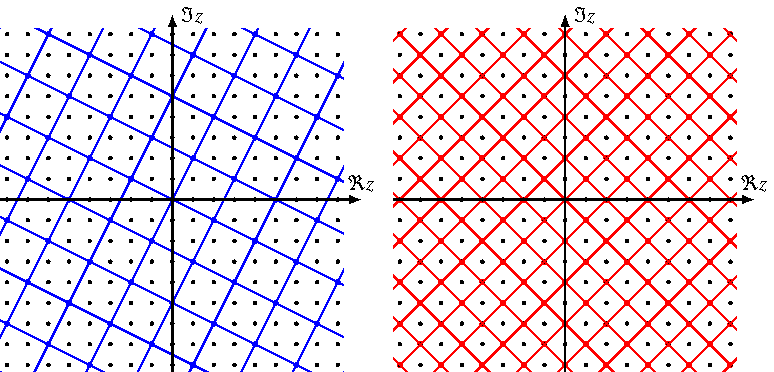
\includegraphics{chapters/10-vektorenmatrizen/images/ideale.pdf}
\caption{Ideale im Ring der ganzen Gaussschen Zahlen $\mathbb{Z}[i]$.
Für jedes Element $r\in \mathbb{Z}[i]$ ist die Menge  $r\mathbb{Z}[i]$
ein ein Ideal in $\mathbb{Z}[i]$.
Links das Ideal $(1+2i)\mathbb{Z}[i]$ (blau), rechts das Ideal
$(1+i)\mathbb{Z}[i]$ (rot).
\label{buch:vektorenmatrizen:fig:ideale}}
\end{figure}
Bei der Betrachtung der additiven Gruppe des Ringes $\mathbb{Z}$ der
ganzen Zahlen wurde bereits die Untergruppe $n\mathbb{Z}$ diskutiert
und die Faktorgruppe $\mathbb{Z}/n\mathbb{Z}$ der Reste konstruiert.
Reste können aber auch multipliziert werden, es muss also auch möglich
sein, der Faktorgruppe eine multiplikative Struktur zu verpassen.

Sei jetzt also $I\subset R$ ein Unterring.
Die Faktorgruppe $R/I$ hat bereits die additive Struktur, es muss
aber auch die Multiplikation definiert werden.
Die Elemente $r_1+I$ und $r_2+I$ der Faktorgruppe $R/I$ haben das
Produkt
\[
(r_1+I)(r_2+I)
=
r_1r_2 + r_1I + Ir_2 + II.
\]
Dies stimmt nur dann mit $r_1r_2+I$ überein, wenn $r_1I\subset I$ und
$r_2I\subset I$ ist.

\begin{definition}
Ein Unterring $I\subset R$ heisst ein {\em Ideal}, wenn für jedes $r\in R$ gilt
$rI\subset I$ und $Ir\subset I$ gilt.
\index{Ideal}%
Die Faktorgruppe $R/I$ erhält eine natürliche Ringstruktur, $R/I$ 
heisst der {\em Quotientenring}.
\index{Quotientenring}%
\end{definition}

\begin{beispiel}
Die Menge $n\mathbb{Z}\subset\mathbb{Z}$ besteht aus den durch $n$ teilbaren
Zahlen.
Multipliziert man durch $n$ teilbare Zahlen mit einer ganzen Zahl,
bleiben sie durch $n$ teilbar, $n\mathbb{Z}$ ist also ein Ideal in
$\mathbb{Z}$.
Der Quotientenring ist der Ring der Reste bei Teilung durch $n$,
er wird in 
Kapitel~\ref{buch:chapter:endliche-koerper}
im Detail untersucht.
\end{beispiel}

Ein Ideal $I\subset R$ drückt als die Idee ``gemeinsamer Faktoren''
auf algebraische Weise aus und der Quotientenring $R/I$ beschreibt
das, was übrig bleibt, wenn man diese Faktoren ignoriert.

\begin{beispiel}
In Abbildung~\ref{buch:vektorenmatrizen:fig:ideale} sind zwei
Ideale im Ring der ganzen Gaussschen Zahlen dargestellt.
Die blauen Punkte sind $I_1=(1+2i)\mathbb{Z}$ und die roten Punkte sind
$I_2=(1+i)\mathbb{Z}$.
Die Faktorgruppen $R/I_1$ und $R/I_2$ fassen jeweils Punkte, die sich
um ein Element von $I_1$ bzw.~$I_2$ unterscheiden, zusammen.

Im Falle von $I_2$ gibt es nur zwei Arten von Punkten, nämlich
die roten und die schwarzen, der Quotientenring hat
daher nur zwei Elemente, $R/I_2 = \{0+I_2,1+I_2\}$.
Wegen $1+1=0$ in diesem Quotientenring, ist $R/I_2=\mathbb{Z}/2\mathbb{Z}$.

Im Falle von $I_1$ gibt es fünf verschiedene Punkte, als Menge ist
\[
R/I_1 
=
\{
0+I_1,
1+I_1,
2+I_1,
3+I_1,
4+I_1
\}.
\]
Die Rechenregeln sind also dieselben wie im Ring $\mathbb{Z}/5\mathbb{Z}$.
In gewisser Weise verhält sich die Zahl $1+2i$ in den ganzen 
Gaussschen Zahlen bezüglich Teilbarkeit ähnlich wie die Zahl $5$ in den
ganzen Zahlen.
\end{beispiel}


%
% algebren.tex -- Grundlegende Konstruktionen für Algebren
%
% (c) 2021 Prof Dr Andreas Müller, OST Ostschweizer Fachhochschule
%
\subsection{Algebren
\label{buch:grundlagen:subsection:algebren}}
Die Skalar-Multiplikation eines Vektorraums ist in einem Ring nicht
vorhanden.
Die Menge der Matrizen $M_n(\Bbbk)$ ist sowohl ein Ring als auch
ein Vektorraum.
Man nennt eine {\em $\Bbbk$-Algebra} oder {\em Algebra über $\Bbbk$}
\index{k-Algebra@$\Bbbk$-Algebra}%
\index{Algebra}%
ein Ring $A$, der auch eine $\Bbbk$-Vektorraum ist.
Die Multiplikation des Ringes muss dazu mit der Skalarmultiplikation
verträglich sein.
Dazu müssen Assoziativgesetze
\index{Assoziativgesetz}
\[
\lambda(\mu a) = (\lambda \mu) a
\qquad\text{und}\qquad
\lambda(ab) = (\lambda a) b
\]
für $a,b\in A$ und $\lambda,\mu\in\Bbbk$
und eine Regel der Form
\begin{equation}
a(\lambda b) = \lambda (ab)
\label{buch:vektorenmatrizen:eqn:algebrakommutativ}
\end{equation}
gelten.
Die Bedingung \eqref{buch:vektorenmatrizen:eqn:algebrakommutativ} ist
eine Folge der Forderung, dass die Multiplikation 
eine lineare Abbildung sein soll.
Dies bedeutet, dass
\begin{equation}
a(\lambda b+\mu c) = \lambda (ab) + \mu (ac)
\label{buch:vektorenmatrizen:eqn:algebralinear}
\end{equation}
ist,
woraus 
\eqref{buch:vektorenmatrizen:eqn:algebrakommutativ}
folgt, indem man
$\mu=0$ setzt.
Die Regel \eqref{buch:vektorenmatrizen:eqn:algebralinear}
beinhaltet aber auch das Distributivgesetz.
$M_n(\Bbbk)$ ist eine Algebra.

\subsubsection{Die Algebra der Funktionen $\Bbbk^X$}
Sei $X$ eine Menge und $\Bbbk^X$ die Menge aller Funktionen $X\to \Bbbk$.
\index{kX@$\Bbbk^X$}%
Auf $\Bbbk^X$ kann man Addition, Multiplikation mit Skalaren und
Multiplikation von Funktionen punktweise definieren.
Für zwei Funktion $f,g\in\Bbbk^X$ und $\lambda\in\Bbbk$ definiert man
\[
\begin{aligned}
&\text{Summe $f+g$:}
&
(f+g)(x) &= f(x)+g(x)
\\
&\text{Skalare $\lambda f$:}
&
(\lambda f)(x) &= \lambda f(x)
\\
&\text{Produkt $f\cdot g$:}
&
(f\cdot g)(x) &= f(x) g(x)
\end{aligned}
\]
Man kann leicht nachprüfen, dass die Menge der Funktionen $\Bbbk^X$
mit diesen Verknüpfungen die Struktur einer $\Bbbk$-Algebra erhält.

Die Algebra der Funktionen $\Bbbk^X$ hat auch ein Einselement:
die konstante Funktion
\[
1\colon [a,b] \to \Bbbk : x \mapsto 1
\]
mit Wert $1$ erfüllt
\[
(1\cdot f)(x) = 1(x) f(x) = f(x)
\quad\Rightarrow\quad 1\cdot f = f,
\]
die Eigenschaft einer Eins in der Algebra.

\subsubsection{Die Algebra der stetigen Funktionen $C([a,b])$}
Die Menge der stetigen Funktionen $C([a,b])$ ist natürlich eine Teilmenge
aller Funktionen: $C([a,b])\subset \mathbb{R}^{[a,b]}$ und erbt damit
auch die Algebraoperationen.
Man muss nur noch sicherstellen, dass die Summe von stetigen Funktionen,
das Produkt einer stetigen Funktion mit einem Skalar und das Produkt von
stetigen Funktionen wieder eine stetige Funktion ist.
Eine Funktion ist genau dann stetig, wenn an jeder Stelle der Grenzwert
mit dem Funktionswert übereinstimmt.
Genau dies garantieren die bekannten Rechenregeln für stetige Funktionen.
Für zwei stetige Funktionen $f,g\in C([a,b])$ und einen Skalar
$\lambda\in\mathbb{R}$ gilt
\[
\begin{aligned}
&\text{Summe:}
&
\lim_{x\to x_0} (f+g)(x)
&=
\lim_{x\to x_0} (f(x)+g(x))
=
\lim_{x\to x_0} f(x) + \lim_{x\to x_0}g(x)
=
f(x_0)+g(x_0) = (f+g)(x_0)
\\
&\text{Skalare:}
&
\lim_{x\to x_0} (\lambda f)(x)
&=
\lim_{x\to x_0} (\lambda f(x)) = \lambda \lim_{x\to x_0} f(x)
=
\lambda f(x_0) = (\lambda f)(x_0)
\\
&\text{Produkt:}
&
\lim_{x\to x_0}(f\cdot g)(x)
&=
\lim_{x\to x_0} f(x)\cdot g(x)
=
\lim_{x\to x_0} f(x)\cdot
\lim_{x\to x_0} g(x)
=
f(x_0)g(x_0)
=
(f\cdot g)(x_0).
\end{aligned}
\]
für jeden Punkt $x_0\in[a,b]$.
Damit ist $C([a,b])$ eine $\mathbb{R}$-Algebra.
Die Algebra hat auch eine Eins, da die konstante Funktion $1(x)=1$ 
stetig ist.






%
% koerper.tex -- Definition eines Körpers
%
% (c) 2021 Prof Dr Andreas Müller, OST Ostschwêizer Fachhochschule
%
\subsection{Körper
\label{buch:subsection:koerper}}
Die Multiplikation ist in einer Algebra nicht immer umkehrbar.
Die Zahlenkörper von Kapitel~\ref{buch:chapter:zahlen} sind also
sehr spezielle Algebren, man nennt sie Körper.
In diesem Abschnitt sollen die wichtigsten Eigenschaften von Körpern
zusammengetragen werden.









